
\begin{problem}{2.3}{problem2_3}
Consider the DC-DC buck converter in Fig. 2.19 which belongs to the class of attenuation circuits; the corresponding dynamic equations are given by:
$$
	\begin{aligned}
		L \frac{d i}{d t} & =-v+u V_{i n}  \\
		C \frac{d v}{d t} & =i-\frac{v}{R}
	\end{aligned}
$$
where $i$ is the current through the inductor $L, v$ is the voltage across the capacitor $C$, $V_{i n}$ is the input voltage, and $u \in\{0,1\}$ is the switching control signal. The goal is to stabilize the output voltage $v$ at the desired level $v_d$. This goal is to be achieved via stabilization of the inductor current $i$ at the desired level $i_d=\frac{v_d}{R}$ using sliding mode control, for this purpose:
(a) Setting $\sigma=i-i_d$ and using the control input $u=\frac{1}{2}(1-\operatorname{sign}(\sigma))$, find the equivalent control and the sliding mode dynamics.
(b) Considering $L=20 \mathrm{mH}, C=20 \mu \mathrm{~F}, R=30 \Omega$, $V_{i n}=15 \mathrm{~V}, v_d=10 \mathrm{~V}$, and the initial conditions $i(0)=0.1 \mathrm{~A}$ and $v(0)=5 \mathrm{~V}$, confirm the efficacy of the controller by simulations.
\end{problem}

\begin{solution}{}{solution2_3}
	\textbf{(a) Equivalent control and sliding mode dynamics}

	\begin{enumerate}
		\item \textbf{State-space representation}

		      Defining the state variables $x_1 = i$ and $x_2 = v$, the system can be written as:

		      $$
			      \begin{aligned}
				      \dot{x}_1 & = -\frac{1}{L}x_2 + \frac{1}{L}uV_{\text{in}} \\
				      \dot{x}_2 & = \frac{1}{C}x_1 - \frac{1}{RC}x_2
			      \end{aligned}
		      $$

		      where the desired current, sliding surface, and control law are given by:

		      $$
			      i_d = x_1^{\star} = \frac{x_2^{\star}}{R}, \quad \sigma = x_1 - x_1^{\star}, \quad u = \frac{1}{2}\left( 1 - \text{sign}(\sigma) \right)
		      $$

		\item \textbf{Equivalent control calculation}

		      The equivalent control $u_{\text{eq}}$ is obtained when $\dot{\sigma} = 0$:

		      $$
			      \begin{aligned}
				      \dot{\sigma} & = \dot{x}_1 - \dot{x}_1^{\star}                                                   \\
				                   & = -\frac{1}{L}x_2 + \frac{1}{L} u V_{\text{in}} - \frac{\dot{x}_2^{\star}}{R} = 0
			      \end{aligned}
		      $$

		      Solving for $u_{\text{eq}}$ yields:

		      $$
			      u_{\text{eq}} = \frac{L}{V_{\text{in}}} \left( \frac{1}{R}\dot{x}_2^{\star} + \frac{1}{L}x_2 \right)
		      $$

		\item \textbf{Sliding mode dynamics}

		      Substituting $u_{\text{eq}}$ into the system dynamics:

		      $$
			      \dot{x}_1 = -\frac{1}{L}x_2 + \frac{1}{L}V_{\text{in}} \cdot \frac{L}{V_{\text{in}}} \left( \frac{1}{R}\dot{x}_2^{\star} + \frac{1}{L}x_2 \right) = \frac{1}{R}\dot{x}_2^{\star}
		      $$

		      Therefore, the sliding mode dynamics are:

		      $$
			      \begin{aligned}
				      \dot{x}_1 & = \frac{1}{R}\dot{x}_2^{\star}     \\
				      \dot{x}_2 & = \frac{1}{C}x_1 - \frac{1}{RC}x_2
			      \end{aligned}
		      $$

		      Note that if $x_1^{\star}$ (or $x_2^{\star}$) is constant, then $\dot{x}_2^{\star} = 0 \Rightarrow \dot{x}_1 = 0$.
	\end{enumerate}

	\textbf{(b) Simulation validation}

	The simulation results using the given parameters are shown below:
	% \begin{figure}[H]
	% 	\centering
	% 	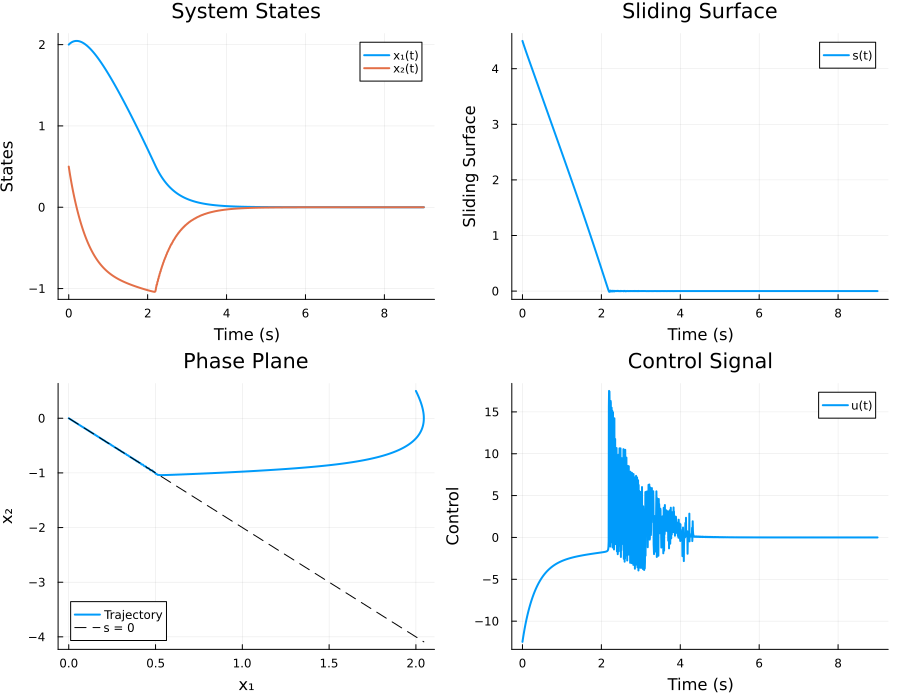
\includegraphics[width=1\textwidth]{img/problem1_2_sigmoid.png}
	% 	\caption{Simulation results for the sliding mode control system using sigmoid approximation.}
	% 	\label{fig:problem1_2_sig}
	% \end{figure}
	\begin{figure}[H]
		\centering
		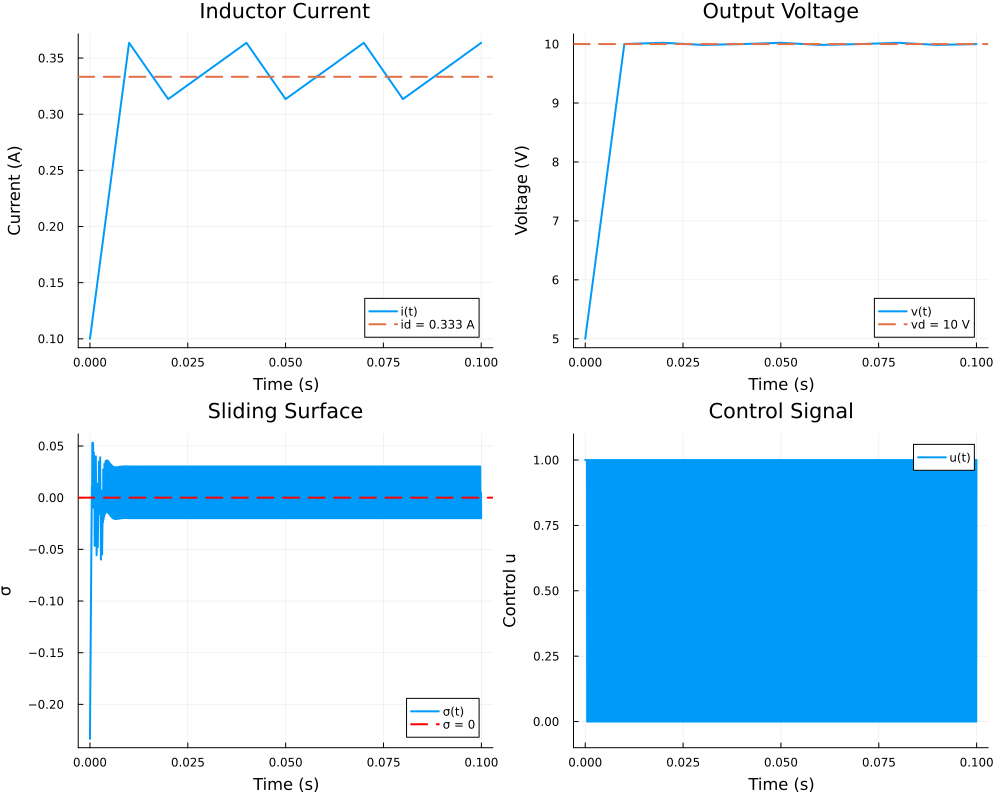
\includegraphics[width=1\textwidth]{img/problem2_3.png}
		\caption{Simulation results for the DC-DC buck converter with sliding mode control.}
		\label{fig:problem2_3}
	\end{figure}

	The simulation confirms the effectiveness of the sliding mode controller, as voltage converge to its desired value ($v_d = 10$ V) within a short time period, also the current oscilates around the desired value ($i_d = 0.3333$ A) and the system is stable. The chattering in the control signal is also evident, which is a common characteristic of sliding mode control systems.
\end{solution}